\section{Methodology}\label{methodology}

Combining the efficiency of ASP languages with the representational power of ANNs is a non-trivial task. Not only does it require a novel representation of the ANN structure, but Clingo has no floating-point support. This requires clever simplifications of the activations functions and gradiant descent to use them over integers. Additionally, large ANNs can cause combinatorial explosions in the search space, making grounding the programs difficult. The C-MCPN Framework and Editor were developed to address some of these challenges, providing a structured way to represent and work with logical networks in Clingo.

\subsection{Domain Selection}

To build and test the framework the illustrative domain of digital logic for hardware development was selected. Its simplicity and familiarity make it an ideal domain for experimentation. 

For our example network, a 1-bit adder seen in Figure \ref{1_bit_adder}, we used neurons with three types of well established logic gates: AND, OR, and XOR. In Table \ref{definition_table} we show the neuron definitions of these gates, and their truth tables. Using a combination of these and more gates, one is able to construct complex logical operations\footnote{An elegant and simple proof of Clingo's Turing completeness falls out of the C-MCPN Framework.}.

\vspace{-10pt}
\begin{table}[h]
% \caption{McCulloch-Pitts Neuron Definitions and Truth Tables.}
\caption{Neuron Definitions and Truth Tables.}
\label{definition_table}
\begin{center}
\fbox{
\begin{tabular}{|cc|c|cc|c|cc|c|}
    \hline
    \multicolumn{3}{|c|}{\textbf{AND}} & \multicolumn{3}{c|}{\textbf{OR}} & \multicolumn{3}{c|}{\textbf{XOR}} \\
    \multicolumn{3}{|c|}{$g(\vec{x}) = x_1 \cdot x_2$} & \multicolumn{3}{c|}{$g(\vec{x}) = x_1 + x_2$} & \multicolumn{3}{c|}{$g(\vec{x}) = |x_1 - x_2|$} \\[1em]
    % \multicolumn{3}{|c|}{$g(\vec{x}) = x_1 \cdot x_2,\ \theta = 1$} & \multicolumn{3}{c|}{$g(\vec{x}) = x_1 + x_2,\ \theta = 1$} & \multicolumn{3}{c|}{$g(\vec{x}) = |x_1 - x_2|,\ \theta = 1$} \\[1em]

    % \hdashline
    % \multicolumn{2}{|c}{} & \multicolumn{3}{c}{Activation: } & \multicolumn{4}{c|}{$f(\vec{x}) = \begin{cases} 0 & \text{if } g(\vec{x}) < \theta,\\ 1 & \text{if } g(\vec{x}) \geq \theta. \end{cases}$} \\[1em]
    % \hdashline

    % \multicolumn{3}{|c|}{AND} & \multicolumn{3}{c|}{OR} & \multicolumn{3}{c|}{XOR} \\
    $x_1$ & $x_2$ & $f(\vec{x})$ & $x_1$ & $x_2$ & $f(\vec{x})$ & $x_1$ & $x_2$ & $f(\vec{x})$ \\
    \hline
    T & T & T & T & T & T & T & T & F \\
    T & F & F & T & F & T & T & F & T \\
    F & T & F & F & T & T & F & T & T \\
    F & F & F & F & F & F & F & F & F \\
    \hline
\end{tabular}
}
\end{center}
\end{table}
\vspace{-10pt}

\begin{figure}[h]
    \centering
    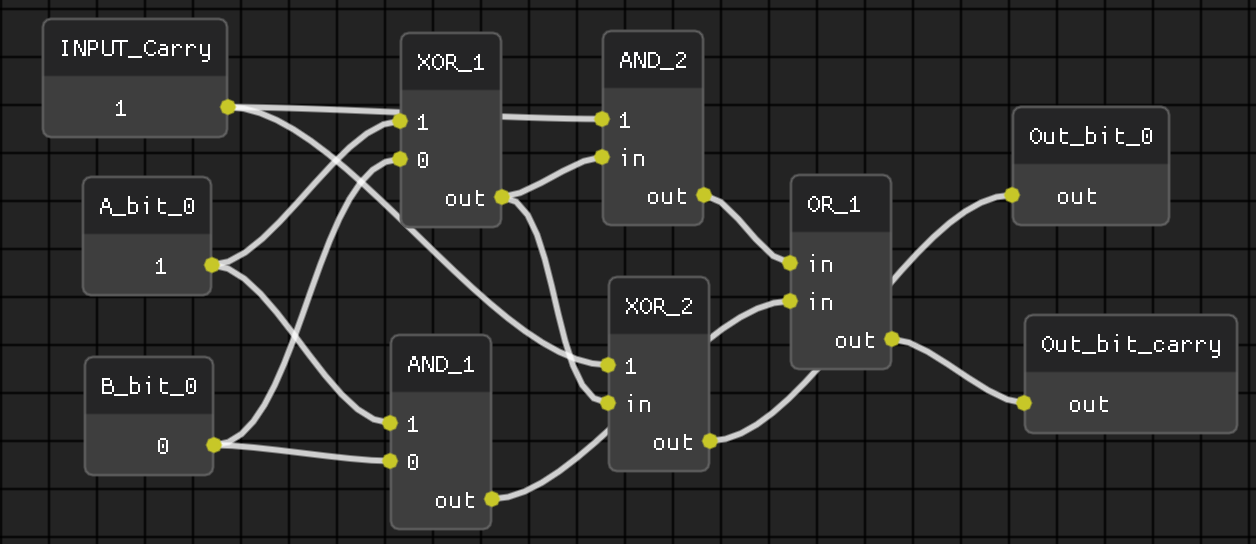
\includegraphics[width=0.6\textwidth]{figures/1-bit adder.png}
    \caption{A screenshot of a 1-bit adder network in the C-MCPN Editor.}
    \label{1_bit_adder}
\end{figure}

\subsection{Design Approach}

The representation of an artificial neuron requries both the \emph{structure} designation, and the function used to \emph{activate} it. When activated the neuron will propagate a signal to its output given the provided input signals. Its value then further propagates through the network along edges and activating other neurons.

An {\tt AND} gate is used to illustrate how we represent an artificial neuron:
\begin{lstlisting}[basicstyle=\ttfamily\small]
% gate(TYPE, OUTPUT, INPUTS)
gate("AND", Out, In1, In2) :- values(In1), values(In2),
                              Out = (In1 * In2).
\end{lstlisting}

The \emph{structure} of the neuron is indicated by the parameters: in the case of an {\tt AND} gate this requires two input parameters and a single output. The \emph{activation function} is encoded directly in the rule structure using the arithmetic equivalent provided in Table \ref{definition_table}.

The neuron \emph{connectivity} specified in the gate definitions can then be used to forge connections of a network. A connection from the 1-bit adder sample network is built as:
\begin{lstlisting}[basicstyle=\ttfamily\small]
% neuron(type, unique_id)
neuron("INPUT", "INPUT_1").
neuron("XOR", "XOR_1").

% edge(source_id, target_id)
edge("INPUT_1", "XOR_1").

% val(neuron_id, value).
val("INPUT_1", 1).
\end{lstlisting}

Finally, the value inference program is used to store the possible values, activate the neurons, and propagate the values through the network. The program for a 2-input gate can be built as:
\begin{lstlisting}[basicstyle=\ttfamily\small]
%% Value domain
values(0;1).

% Edges carry values from input to output
edge(In, Neuron_id, Val) :-
    edge(In, Neuron_id),
    neuron(_, Neuron_id),
    neuron(_, In),
    val(In, Val).

% 2 input gates
val(Neuron_id, Val) :-
    gate(Type, Val, Val1, Val2),
    neuron(Type, Neuron_id),
    edge(In1, Neuron_id, Val1),
    edge(In2, Neuron_id, Val2),
    In1 != In2.

%% Each neuron has one value
{ val(Neuron_id, Val) : values(Val) } 1 :- neuron(_, Neuron_id).

%% Show values
#show val/2.
\end{lstlisting}

The rule carrying the values along the edges is vital to the functioning of the network. Without it, the network gets "stuck" and is unable to infer what the values should be. This is a key insight we had during development.
